\documentclass{article}
\usepackage[utf8]{inputenc}
\usepackage{amsmath}
\usepackage{amsfonts}
\usepackage{xcolor}
\DeclareMathOperator*{\argmax}{arg\,max}
\DeclareMathOperator*{\argmin}{arg\,min}

\title{Investigation of Reinforcement Learning Methods for Raceline Optimization (Attempt)}
\author{Joseph Hadidjojo, Tung Pham}
\date{\today}
% \date{\vspace{-1em}}

\usepackage{natbib}
\usepackage{graphicx}
\usepackage{url}

\begin{document}

\maketitle

% for final report only
\begin{abstract}
	%A one paragraph high level description of the work. The abstract is typically the first thing someone would read from the paper before deciding whether to continue reading and hence, serves as an advertisement to the reader to read the whole paper. 
    This work initially attempts to investigate the application of reinforcement learning (RL) to optimize raceline trajectories. However, due to unexpected complications in the environment setup, the RL agents were tested on the CartPole environment instead. The performance of Deep Q-Networks (DQN) and Double Deep Q-Networks (DDQN) were compared. DQN exhibited rapid early learning but suffered from long-term instability due to overestimation bias. In contrast, DDQN demonstrated smoother learning, sustained optimal performance, and improved stability. These results validate the theoretical advantages of DDQN and highlight its suitability for solving complex problems like raceline optimization. However, further work is needed to develop a representative raceline optimization environment to fully evaluate and conclusively confirm its applicability.
\end{abstract}

% \begin{abstract}
% This project investigates the application of reinforcement learning (RL) to optimize raceline trajectories. Due to unexpected complications, the agents were tested on the CartPole environment, chosen for its similar state representations and underlying physics. The study compared the performance of Deep Q-Networks (DQN) and Double Deep Q-Networks (DDQN). DQN exhibited rapid early learning but suffered from long-term instability due to overestimation bias. In contrast, DDQN demonstrated smoother learning, sustained optimal performance, and improved stability. These results validate the theoretical advantages of DDQN and highlight its potential suitability for solving complex problems like raceline optimization. Future work will focus on developing a representative raceline optimization environment and leveraging transfer learning to adapt agents for real-world systems like the F1Tenth platform.
% \end{abstract}



\section{Introduction}

Formula 1 (F1) racing is renowned for the intense precision, skill, and strategy that its drivers bring to the track. In each race, drivers must determine the fastest path around the circuit, or the "racing line," which enables them to maintain optimal speed while negotiating corners and straights. This process is not merely a physical feat; it requires an in-depth understanding of the vehicle's capabilities and a sharp sense of timing. Talented drivers often master the racing line in only a few laps of practice, fine-tuning it to suit their unique driving style and the distinct characteristics of their machinery \cite{brouillard2016perfectcorner}.

Inspired by this mastery, the objective of this work is to explore the potential of reinforcement learning (RL) to approximate an optimal racing line on a simplified racing track. The core idea is to use RL, where an agent learns through experience, to find the fastest path around a track by optimizing two key actions: acceleration and rotation. By framing the problem in this way, we aim to develop a model that could eventually serve as a foundational tool for amateur racers with limited experience.

However, this problem presents unique challenges compared to more conventional RL problems:

\begin{itemize}
	\item \textbf{High-dimensional state and action spaces}: Unlike simpler tasks with discrete or limited action spaces, racing involves continuous control of speed, position, and rotation, all of which must be adjusted dynamically to adapt to the track layout.

	\item \textbf{Balancing competing objectives}: Achieving the optimal racing line requires the agent to balance maximizing speed with avoiding crashes, spin-outs, and leaving the track boundaries. High speeds, especially around tight corners, increase the risk of the agent veering off course, demanding precise control over acceleration and rotation to maintain the ideal path within the track’s limits.

	\item \textbf{Delayed rewards}: The consequences of an action, like setting up for a corner, may not be immediately evident. The agent must learn to associate actions taken several turns ago with the eventual outcome, making the learning process more complex.

	\item \textbf{Track variability and precision demands}: Unlike simpler environments, the race track’s varying curvature and the need for fine-grained control make it harder for the agent to generalize its learned strategy across different segments of the track.
\end{itemize}

These factors contribute to making the problem of finding an optimal race line particularly challenging, setting it apart from simpler RL applications.

While F1 and professional racing teams likely already utilize advanced tools and systems to estimate the optimal racing line, these applications are typically proprietary and remain restricted to private use. Due to the competitive nature of the sport, insights and strategies derived from such systems are rarely disclosed to the public. Consequently, amateur racers and enthusiasts have limited access to data-driven methods for learning and improving their racing lines. By exploring this problem with reinforcement learning, we aim to create a foundation for a more accessible tool that can help individuals develop their skills and gain insights into racing line optimization without requiring the high costs or exclusivity of professional-grade systems/academies. This work not only contributes to the field of RL in complex control tasks but also has the potential to democratize access to advanced racing analytics for a broader audience.

\section{Background and Related Works}

Reinforcement learning (RL) has seen significant advancements in recent years, especially in applications requiring continuous control and dynamic decision-making, such as autonomous driving and racing. In racing, RL agents must optimize not only for speed but also for stability, as they navigate complex tracks with tight turns and variable conditions. This section reviews notable works in RL and autonomous driving that have informed the development of driving and racing agents, highlighting the techniques and challenges relevant to this project.

\subsection{Deep Q-Network (DQN)}
A foundational work in deep reinforcement learning is the introduction of the Deep Q-Network (DQN) by Mnih et al. (2015) \cite{mnih2015human}, which achieved human-level performance on Atari games. Although the DQN algorithm primarily focuses on discrete action spaces, it inspired adaptations for continuous and complex environments, such as autonomous driving and racing, where agents must navigate through tracks while balancing speed and control. This approach laid the groundwork for subsequent RL algorithms that could handle the continuous control demands of racing tasks.

\subsection{Double Deep Q-Network (DDQN)}
Double Deep Q-Networks (DDQN), proposed by van Hasselt et al. (2016) \cite{van2016deep}, addressed the overestimation bias in DQN by decoupling action selection and action evaluation. In DDQN, the next action is selected using the current Q-network, while its value is evaluated using the target network, resulting in more accurate target Q-values. This improvement enhances stability and policy performance, particularly in environments with high-dimensional state spaces and delayed rewards. DDQN’s robustness makes it especially relevant to racing tasks, where balancing speed and control is critical.

\subsection{Learning to Drive in a Day}
Kendall et al. (2018) demonstrated the application of deep reinforcement learning to autonomous driving by training a model to perform lane following in a synthetic environment, followed by transferring the learned policy to a real-life driving environment \cite{kendall2018drive}. Their approach utilized a model-free reinforcement learning algorithm, with all exploration and optimization conducted directly on the vehicle. This work highlighted the potential of end-to-end learning systems in autonomous driving, moving away from reliance on predefined rules and maps. 
% The state representation, which combined visual input with vehicle dynamics, inspired the formulation of state representations in our project, emphasizing the integration of sensory data for effective decision-making in reinforcement learning frameworks.


% \subsection{Racing Agent with Reinforcement Learning}
% In racing, agents often benefit from continuous-action reinforcement learning algorithms, which allow finer control over movement variables such as speed and rotation. The Soft Actor-Critic (SAC) algorithm, introduced by Haarnoja et al. (2018) \cite{haarnoja2018soft}, is well-known for its ability to handle continuous action spaces with entropy regularization. SAC’s exploration techniques are possibly quite effective for racing environments, where agents must strike a balance between fast exploration of new actions and reliable, safe driving.

% \subsection{Using RL for Track Navigation in Self-Driving Cars}
% Another significant contribution to continuous-action reinforcement learning is the Deep Deterministic Policy Gradient (DDPG) algorithm by Lillicrap et al. (2016) \cite{lillicrap2015continuous}. DDPG has shown promise in applications requiring high-precision control. By enabling continuous state and action spaces, DDPG provides a foundation for control in dynamic and high-stakes environments, which we believe makes it well-suited for racing agent applications.

By drawing on these established techniques, this project seeks to develop an RL-based racing agent capable of navigating a simplified F1 track while balancing speed and stability, making it accessible as a foundational tool for aspiring racers.

% Following, you should provide the necessary background and discuss related work in the RL literature. This section should also be about a page. Citations should be in BibTeX format \citep{thrun2005probabilistic}.

\section{Technical Approach / Methodology / Theoretical Framework}

% for proposal
%Describe how you will approach the problem and its technical formulation. Feel free to re-state the basic RL formulas (e.g., if using Q-learning, state the update rule or the formula for what the Q function approximates). 

% for final report
\subsection{Problem Formulation}
% \subsubsection{Formulation}

We envision our agent to operate within a discrete racing track environment represented as a 2D space.
At each time step \(t\), the agent observes the current state \(s_t\), which includes:
\begin{itemize}
	\item Car Position on the track (\(x, y\)),
	\item Car Velocity components (\(v_x, v_y\)),
	\item Car Orientation (\(\theta\)),
	\item Car Angular momentum (\(\omega\)),
	\item Car's Absolute distance to Left and Right track limits
\end{itemize}

The agent selects an action \(a_t = [a_{\text{acc}}, a_{\text{rot}}]\), where:
\begin{itemize}
	\item \(a_{\text{acc}}\) controls acceleration, constant (do nothing) or deceleration (\(a\in\{-1,
	      0, 1\}\)),
	\item \(a_{\text{rot}}\) controls the steering angle of the car from full-left, neutral or full-right
	      (\(\Delta\theta\in\{-1, 0, 1\}\))
\end{itemize}

The environment updates the agent’s state based on these actions and the track's physics, such as track boundaries.
Most real-life environmental factors such as friction, elevation, and grip condition will be ignored.
The agent receives a reward \(r\) at the end of each lap, formulated as 
\[ 
r = -T +\alpha\Delta v_{max} - \beta O 
\] 
where $T$ is the lap time, $\Delta v_{max}$ is the maximum speed change over a run, $O$ is the number of track excursions, and $\alpha$, $\beta$ are tunable weight parameters.
% \begin{itemize}
% 	\item $T$ is the lap time.
% 	\item $\Delta v_{max}$ is the maximum speed change over a run.
% 	\item $O$ is the number of track excursions.
% 	\item $\alpha$, $\beta$ are tunable weight parameters.
% \end{itemize}
Through this, the agent learns to balance the objectives of speed and control (reducing spin-outs and track excursions), gradually improving its policy over training episodes.

\subsubsection{Major Roadblock}

Initially, we had selected the Car Racing v2 environment from Gymnasium v1.0 as the prime candidate for our agent's testing environment. However, we discovered that there was a bug in the discrete version of the environment that crashed the environment whenever it was initialized. 
Committing to this environment would result in an extensive effort to debug and develop a fix, in addition to adapting the environment to our current problem formulation. This resulted in a severe underestimation of the amount of work required to set up our environment as desired. 

Due to the time and resource constraints, and upon consultation with the course instructor Yash Shukla, a decision was made to instead test our algorithm implementation on an alternative environment. To this end, Gymnasium's Cart Pole environment was selected due to its similar state-space representation and underlying physics formulation as our envisioned Problem Formulation.

\subsubsection{Gymnasium's CartPole Environment}

In this environment, the agent operates within a discrete space where at each
time step $t$, the agent observes the current state $s_t$, which includes the
followings:
\begin{itemize}
	% \item Cart Position, $p$, on the x-axis ($-4.8 < p < 4.8$)
    \item Cart Position ($p$) on the x-axis,
	\item Cart Velocity ($v$),
	\item Pole Angle ($\theta$),
	\item Pole angle velocity ($\omega$)
\end{itemize}

The actions that the agent can take at any given time $t$ is to push the cart with a fixed amount of force in either the left or right direction ($a \in \{0, 1\})$.
% where $0$ represents pushing the cart to the left, and $1$ represents pushing the cart to the right.
% where
% \begin{itemize}
% 	\item 0: push the cart to the left.
% 	\item 1: push the cart to the right.
% \end{itemize}

The environment will then perform the underlying physics calculation needed (such as the velocity impact based on the angle of the pole) and update the state based on the action taken. Most real-life environmental factors, such as friction, are ignored. The agent receives 1 unit of reward for every timestep the pole is kept upright.

\subsection{Methodology}
To optimize the agent’s behavior, we leverage two reinforcement learning techniques: Deep Q-Networks (DQN) and Double Deep Q-Networks (DDQN). Each method builds upon fundamental principles of RL, such as the Bellman equation and policy optimization.

% \subsubsection{Deep Q Network}

% Q-Learning algorithm in Sutton and Barton has significant limitations when applied to complex environments:

\subsubsection{Q-Learning and Deep Q-Learning} \label{sec:Q_deepQ_learn}

\textbf{Q-learning} \cite{watkins1989learning} is a value-based reinforcement learning algorithm that seeks to learn the optimal action-value function \(Q^*(s, a)\) using the Bellman equation:
\[
Q^*(s, a) = r + \gamma \max_a Q^*(s', a),
\]
where \(s'\) is the next state, and \(\gamma\) is the discount factor.

The algorithm iteratively updates the Q-values using \cite{sutton1998reinforcement}:
\[
Q(s, a) \leftarrow Q(s, a) + \alpha \left[ r + \gamma \max_a Q(s', a) - Q(s, a) \right],
\]
where \(\alpha\) is the learning rate. This simple, table-based approach works well in discrete environments with small state and action spaces. However, Q-learning has significant limitations when applied to complex environments like racing tracks:

\begin{itemize}
	\item \textbf{High-dimensional state spaces}: Representing continuous states (e.g., positions, velocities, and orientations) as discrete states leads to a combinatorial explosion in the size of the Q-table.
	\item \textbf{Inefficient learning}: In large state-action spaces, learning becomes computationally expensive, and generalization across similar states becomes practically impossible.
	\item \textbf{Overestimation bias}: During training, the agent is prone to picking up noises in the environment which causes the estimated value of some actions to be inflated and propagated, leading to overestimation.
\end{itemize}

These limitations necessitate scalable approaches like \textbf{Deep Q-Networks (DQN)} \cite{mnih2015human} for handling high-dimensional state spaces.
DQN extends Q-learning by approximating the Q-function \(Q(s, a)\) with a deep neural network, enabling it to handle large, high-dimensional state spaces.
Instead of maintaining a Q-table, DQN uses a neural network parameterized by \(\theta\) to predict \(Q(s, a)\) for each possible action. This makes DQN effective for high-dimensional problems, though it remains limited to discrete action spaces.

% DQN introduces two key techniques to improve stability and efficiency:
% \begin{itemize}
% 	\item \textbf{Experience replay}: The agent stores past transitions \((s, a, r, s')\) in a replay buffer. During training, mini-batches of transitions are sampled randomly, reducing correlations between consecutive updates and improving data efficiency.
% 	\item \textbf{Target networks}: A separate target network \(Q(s', a'; \theta^-)\) is used for calculating target Q-values. The parameters \(\theta^-\) are updated periodically to reflect the weights of the current Q-network, reducing the risk of divergence during training.
% \end{itemize}

A key feature introduced by DQN is the \textbf{Experience Replay} memory, a mechanism where the agent stores its past experiences \((s, a, r, s')\) in a replay buffer and samples mini-batches of these experiences randomly to train the network. The Experience Replay is a necessary by-product of leveraging deep neural networks, due to their requirements of independent and identically distributed (i.i.d.) data to be trained effectively (which is not naturally the case for many RL methods, such as the Q-table).

To train the Q-network, DQN minimizes the temporal difference (TD) loss:
\[
	L(\theta) = \mathbb{E}_{(s, a, r, s')} \left[ \left( r + \gamma \max_{a'} Q(s', a'; \theta^-) - Q(s, a; \theta) \right)^2 \right],
\]
where:
\begin{itemize}
	\item \(\theta\): Represents the parameters (weights) of the current Q-network used to approximate \(Q(s, a)\).
	\item \(\theta^-\): Represents the parameters of the target Q-network, which are periodically updated to match \(\theta\). The use of \(\theta^-\) ensures stability by decoupling the target computation from the current network’s rapidly changing parameters.
\end{itemize}

In this work, we leverage the ML framework PyTorch to construct the Deep Q-Network. A 3 fully connected layers network with ReLu activation method was utilized to leverage a simplistic design. Additionally, we incorporate a separate but identical network with delayed weight updates in order to stabilize the training of the Q-Network \cite{towardsdatascience_dqn}.

While DQN is effective for high-dimensional discrete action problems, it still suffers from the same issue of overestimation bias as Q-Learning. This occurs because DQN uses the maximum estimated Q-value \( \max_{a} Q(s', a) \) of the next state \( s' \) for updating the Q-value of the current state-action pair \( Q(s, a) \). If the estimated Q-values are noisy, this approach can systematically overestimate the true values, leading to suboptimal policies and slower convergence. To overcome this issue, Double Deep Q-Network is utilized and will be discussed in further detail in the next section.


\subsubsection{Double Q-Learning and Double Deep Q-Learning} \label{sec: DDQ_learn}
% - To overcome overestimation bias in Q-Learning, one of the approach was to use Double Q-Learning by introduce and maintain a different Q table.
% - Both Q tables overestimate is highly unlikely.
% - Motivated by this Algorithm, Double DQN
% - Very similar to DQN and the only difference was in the way we use the target
% - Use the same network architecture
% network.
% - During training, use current policy network to predict Q value for action
% selection but evaluating this Q prediction with the target network.
% To overcome the overestimation bias in Q-Learning, Sutton and Barton introduce the \textbf{Double Q-Learning} algorithm \cite{sutton1998reinforcement}.
\textbf{Double Q-Learning} \cite{van2010double} was introduced as a method to combat the overestimation bias problem in Q-Learning.
% Similar to Q-Learning, Double Q-Learning is a value-based reinforcement learning algorithm that seeks to learn the optimal action-value function $Q*(s,a)$.
% However, instead of maintaining a single table to store the Q values, it adds an additional table and the algorithm iteratively updates the Q-values using:
It does this by maintaining an additional Q-table estimates and alternates between using one to select the best action and the other to evaluate it. The following update algorithm allows concurrent learning of different estimates simultaneously \cite{sutton1998reinforcement}:
\[
Q_i(S_t, A_t) \leftarrow Q_i(S_t, A_t) + \alpha[R_{t+1} + \gamma Q_j(S_{t+1}, \argmax_{a} Q_i(S_{t+1}, a)) - Q_i(S_t, A_t)]
\]
In the event that one Q-table is overestimating, it is extremely unlikely for the other Q-table to do the same. Therefore, by using one table to update the other, an unbiased estimate can be produced which avoids overestimation.

This approach works well with small and simple environments with limited state and action space.
However, for bigger problems, it faces the same issues as other tabular-based approaches like Q-Learning, as was discussed in \S \ref{sec:Q_deepQ_learn}.

To combine Double Q-Learning's capabilities in mitigating overestimation bias, and the scalability of Deep Q-Networks, the \textbf{Double Deep Q-Networks (DDQN)} \cite{van2016deep} was introduced.
DDQN extends Double Q-Learning by replacing both Q-tables with deep neural networks (commonly referred to as the "online"($\theta$) and "target" ($\theta^-$) network), enabling it to handle much larger and higher-dimensional state spaces. This also improves the original DQN implementation by decoupling the action selection and action evaluation processes, which combined results in a scalable method with minimal overestimation bias.

% \paragraph{Core Idea}

In finer detail: Instead of directly using the maximum Q-value from a single network for the next state \( s' \), DDQN splits the computation into two parts:
\begin{enumerate}
    \item \textbf{Action Selection:} The action \( a^* \) for the next state \( s' \) is chosen using the current (online) Q-network $\theta$:
    \[
    a^* = \arg\max_{a} Q(s', a; \theta).
    \]
    \item \textbf{Action Evaluation:} The value of this action \( Q(s', a^*; \theta^-) \) is then estimated using the target network:
    \[
    Q(s, a) \leftarrow Q(s, a) + \alpha \left[ r + \gamma Q(s', a^*; \theta^-) - Q(s, a) \right].
    \]
\end{enumerate}

By separating the networks used for action selection and evaluation, DDQN avoids the optimistic bias inherent in using a single network for both, thus yielding more accurate Q-value estimates. The reduced bias in Q-value estimates leads to more stable training and faster convergence, particularly in environments with high-dimensional state and action spaces, such as racing tracks. These more accurate Q-value estimates also enable the agent to select more optimal actions, improving overall performance.

In terms of implementation, we once again leverage the PyTorch ML framework and followed the same neural network architectures as our DQN implementation for both of DDQN's Deep Q-Networks (please refer back to \S \ref{sec:Q_deepQ_learn} and the attached codebase for further details).

% \paragraph{Advantages of DDQN}
% \begin{enumerate}
%     \item \textbf{Reduced Overestimation Bias:} By decoupling action selection and evaluation, DDQN ensures that noisy estimates of \( Q(s, a) \) do not propagate through the update process.
%     \item \textbf{Improved Stability:} The reduced bias in Q-value estimates leads to more stable training and faster convergence, particularly in environments with high-dimensional state and action spaces, such as racing tracks.
%     \item \textbf{Better Policy Performance:} The more accurate Q-value estimates enable the agent to select actions that are closer to optimal, improving overall policy performance.
% \end{enumerate}

% \paragraph{Implementation in PyTorch}

% The implementation of DDQN in PyTorch follows a structure similar to that of DQN, with a key modification in the Q-value update process to decouple action selection and evaluation. Below is a high-level description of the key components:

% \begin{enumerate}
%     \item \textbf{Q-Network Architecture:}
%     \begin{itemize}
%         \item A neural network is used to approximate the Q-function \( Q(s, a; \theta) \). The architecture typically consists of fully connected layers with ReLU activation functions.
%         \item A second, identical network (the \textit{target network}) is maintained to compute the target Q-values. Its weights \( \theta^- \) are periodically updated to match the main network's weights \( \theta \).
%     \end{itemize}
%     \item \textbf{Experience Replay:}
%     \begin{itemize}
%         \item Transitions \((s, a, r, s')\) are stored in a replay buffer.
%         \item During training, a mini-batch of transitions is sampled randomly from the buffer to break correlations in the data.
%     \end{itemize}
%     \item \textbf{Action Selection (Current Network):}
%     \[
%     a^* = \arg\max_{a} Q(s', a; \theta).
%     \]
%     \item \textbf{Action Evaluation (Target Network):}
%     \[
%     Q_{\text{target}} = r + \gamma Q(s', a^*; \theta^-).
%     \]
%     \item \textbf{Loss Computation:}
%     \[
%     L(\theta) = \frac{1}{N} \sum_{i=1}^{N} \left( Q_{\text{target}, i} - Q(s_i, a_i; \theta) \right)^2.
%     \]
%     \item \textbf{Target Network Updates:}
%     \begin{itemize}
%         \item Periodically, the weights of the target network are updated to match those of the current network:
%         \[
%         \theta^- \leftarrow \theta.
%         \]
%     \end{itemize}
% \end{enumerate}

% \paragraph{High-Level PyTorch Workflow}
% \begin{itemize}
%     \item \textbf{Initialize Networks:}
%     \begin{itemize}
%         \item Define two instances of the Q-network (current and target) using \texttt{torch.nn.Module}.
%         \item Set up an optimizer (e.g., \texttt{Adam}) for the current network.
%     \end{itemize}
%     \item \textbf{Experience Replay Buffer:}
%     \begin{itemize}
%         \item Implement a buffer to store transitions and sample mini-batches for training.
%     \end{itemize}
%     \item \textbf{Training Loop:}
%     \begin{itemize}
%         \item For each sampled mini-batch:
%         \begin{enumerate}
%             \item Compute $a^*$ using the current network: \texttt{argmax(Q(s', a; θ))}.
%             \item Compute $Q_{\text{target}}$ using the target network for $a^*$.
%             \item Calculate the loss: \texttt{torch.nn.functional.mse_loss}.
%             \item Perform backpropagation to update $\theta$: \texttt{loss.backward()} and \texttt{optimizer.step()}.
%         \end{enumerate}
%     \end{itemize}
%     \item \textbf{Target Network Update:}
%     \begin{itemize}
%         \item Periodically copy the weights of the current network to the target network:
%         \begin{verbatim}
%         target_net.load_state_dict(current_net.state_dict())
%         \end{verbatim}
%     \end{itemize}
% \end{itemize}

% This implementation ensures that the DDQN framework can efficiently decouple action selection and evaluation, leveraging PyTorch’s efficient tensor operations and automatic differentiation for scalable and stable training.

% \paragraph{Comparison with DQN}

% The advantages of DDQN over DQN were particularly evident in preliminary experiments, where DDQN achieved:
% \begin{itemize}
%     \item \textbf{Faster Convergence:} Training stabilized more quickly compared to DQN due to reduced noise in Q-value estimates.
%     \item \textbf{Improved Policy Robustness:} The learned policy was less prone to making risky decisions based on inflated Q-values, resulting in fewer track excursions and smoother lap times.
% \end{itemize}

% This improvement demonstrates the potential of DDQN to handle the nuanced balance between speed and control required for race line optimization.

\subsubsection{Hyperparameter Search}
For both agents, we utilized Python's Ray Tuning package to run a hyperparameter search on two separate machines: an x64-based machine with $10$ concurrent threads and $1$ RTX 3070 GPU with CUDA 12.4 accelerator, and an ARM64-based MPS accelerated computer with $10$ concurrent threads. The hyperparameter search space is defined in Table \ref{tab:hyperparameter_search_space}.
% \begin{itemize}
% 	\item Replay buffer size: [5000, 10000, 20000].
% 	\item Batch size: [64, 128, 256].
% 	\item Starting $\epsilon$: Uniformly selected from 0.9 to 1.0.
% 	\item Minimum $\epsilon$: Uniformly selected from 0.01 to 0.1.
%   \item $\epsilon$ decay rate: [500, 1000, 2000],
%   \item $\tau$: Uniformly selected from $\log{10}{1e-3}$ to $\log{10}{1e-2}$,
% 	\item $\gamma$: Uniformly selected from 0.95 to 0.99.
% 	\item Learning rate: Uniformly selected from $\log{10}{1e-4}$ to $\log{10}{1e-3}$.
% \end{itemize}
\begin{table}[!ht]
\centering
\begin{tabular}{|l|l|}
\hline
\textbf{Hyperparameter} & \textbf{Search Space}     \\ \hline
Replay Buffer Memory    & \{5000, 10000, 20000\}    \\ \hline
Batch Size  & \{64, 128, 256\}          \\ \hline
Starting $\epsilon$     & Uniformly selected from [0.9, 1.0]    \\ \hline
Minimum $\epsilon$      & Uniformly selected from [0.01, 0.1]   \\ \hline
$\epsilon$ Decay Rate   & \{500, 1000, 2000\}   \\ \hline
$\tau$  & Uniformly selected from $\log_{10}(1e^{-3})$ to $\log_{10}(1e^{-2})$  \\ \hline
$\gamma$    & Uniformly selected from [0.95, 0.99]  \\ \hline
Learning Rate   & Uniformly selected from $\log_{10}(1e^{-4})$ to $\log_{10}(1e^{-3})$  \\ \hline
\end{tabular}
\caption{Hyperparameter Search Space. Here $\tau$ is the soft update parameter used to control how quickly the target network's weights are updated to match the main network's weights, $\gamma$ is the discounted factor, and $\epsilon$ is the exploration-exploitation rate used in $\epsilon$-greedy action selection method.}
\label{tab:hyperparameter_search_space}
\end{table}
% Where $\tau$ is the soft update parameter used to controls how quickly the
% target network's weights are updated to match the main network's weights,
% $\gamma$ is the discounted factor, and $\epsilon$ is the
% exploration-exploitation rate used in $\epsilon$-greedy action selection method.
The number of episodes was kept fixed at $1000$ and we formulate our hyperparameter search objective to be the average reward over the last-100 episodes, as well as an additional stability score measured through tracking the minimum reward acquired by the agent over the same period.

% for final report
\section{Experimental Results / Technical Demonstration}
\subsection{Hyperparameter Search Result}
% Our hyperparameter search ran for over 20 minutes for DQN and 2 hours for DDQN, resulting in the following configuration that achieved 500 average rewards convergence at the last 100 episodes and a stability score of 500 for both:
% \begin{itemize}
%     \item DQN:
%         \begin{itemize}
%             \item memory size: 5000
%             \item batch size: 256
%             \item epsilon start: 0.9547764258638659
%             \item epsilon min: 0.030782747461299144
%             \item epsilon decay: 2000
%             \item tau: 0.0038257988709783424
%             \item gamma: 0.9728274544297701
%             \item learning rate: 0.00017850475881509242
%         \end{itemize}
%     \item DDQN:
%         \begin{itemize}
%             \item memory size: 20000,
%             \item batch size: 64,
%             \item epsilon start: 0.9550918958252147,
%             \item epsilon min: 0.0022462275686354082,
%             \item epsilon decay: 3500,
%             \item tau: 0.004220863196126302,
%             \item gamma: 0.9740520048831592,
%             \item learning rate: 0.00034327793534851507,
%         \end{itemize}
% \end{itemize}

The resulting hyperparameter configurations from the search are tabulated in Table \ref{tab:hyperparameters_result}. Both configurations achieved 500 average rewards convergence and a stability score of 500 over the last-100 episodes.
\begin{table}[!ht]
\centering
\begin{tabular}{|l|l|l|}
\hline
\textbf{Parameter}  & \textbf{DQN}  & \textbf{DDQN} \\ \hline
Replay Buffer Memory         & 5000          & 20000         \\ \hline
Batch Size          & 256           & 64            \\ \hline
Starting $\epsilon$    & 0.9548        & 0.9551        \\ \hline
Minimum $\epsilon$      & 0.03078       & 0.002246      \\ \hline
$\epsilon$ Decay Rate    & 2000          & 3500          \\ \hline
$\tau$              & 0.003826      & 0.004221      \\ \hline
$\gamma$            & 0.9728        & 0.97405       \\ \hline
Learning Rate       & 0.0001785     & 0.0003433     \\ \hline
\end{tabular}
\caption{Hyperparameter Search Results for DQN and DDQN}
\label{tab:hyperparameters_result}
\end{table}

\begin{figure}[!ht]
    \centering
    \begin{tabular}{c c}    
    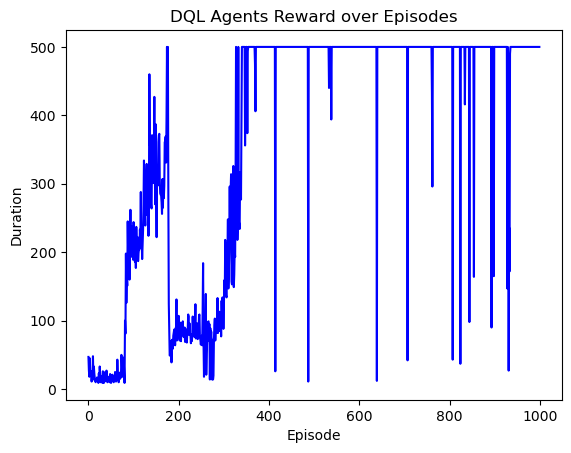
\includegraphics[width=0.45\textwidth]{DQN_rewards.png}
    &
    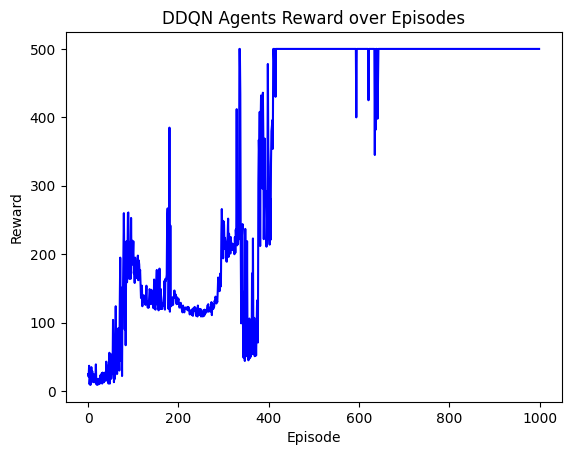
\includegraphics[width=0.45\textwidth]{DDQN_rewards.png}
    \end{tabular}
    % \caption{\color{red}\textbf{Key result 1.} TO EXPLAIN LP-FT OVERFITTING, NEED BETTER CAPTION}
    \caption{Rewards plot over 1000 episodes: DQN (left) and DDQN (right)}
    \label{figure: diag_plot_lpft}
\end{figure}

\subsection{Performance of DQN and DDQN on the CartPole Environment}

The performance of Deep Q-Network (DQN) and Double Deep Q-Network (DDQN) agents on the CartPole environment was evaluated over 1000 episodes by tracking the total rewards achieved. The reward corresponds to the duration for which the agent successfully balances the pole without failure.\footnote{Recorded demonstrations of each method are available at: \url{https://drive.google.com/drive/folders/1zNHzl44QasyTJddteCR-xB4u2pGK30rb?usp=sharing}}

% \subsection{DQN Results}

The DQN agent initially demonstrates a rapid increase in performance, achieving near-optimal rewards by approximately episode 300. However, as training progresses, significant instability emerges. After reaching the maximum reward of 500, the agent frequently experiences sharp drops in performance, where rewards occasionally fall to near-zero values. This inconsistency persists throughout the later episodes, particularly beyond episode 500, highlighting DQN’s struggle to maintain stable and reliable performance. This behavior is attributed to the overestimation bias limitation as discussed in \S\ref{sec:Q_deepQ_learn}. The inflated Q-value estimates introduce instability causing the abrupt fluctuations in rewards.

% This behavior can be attributed to \textbf{overestimation bias}, a known limitation of DQN. By using the same network for both action selection and evaluation, DQN tends to overestimate Q-values, favoring suboptimal actions and leading to erratic updates. These inflated Q-value estimates introduce instability, as seen in the abrupt fluctuations in rewards.

% \subsection{DDQN Results}

In contrast, the DDQN agent shows a smoother and more gradual learning curve. While it takes slightly longer to achieve high rewards compared to DQN, the DDQN agent steadily improves its performance, converging to the maximum reward of 500 by approximately episode 400. Notably, once this optimal performance is reached, the DDQN agent maintains it with remarkable consistency throughout the remaining episodes, exhibiting only minor fluctuations. This improved stability of DDQN can be attributed to its ability to mitigate overestimation bias, as was discussed in \S\ref{sec: DDQ_learn}. By decoupling action selection from value evaluation, DDQN ensures more accurate Q-value estimates, allowing the agent to learn a robust and reliable policy.

% The improved stability of DDQN can be attributed to its ability to mitigate overestimation bias. By decoupling action selection, which is handled by the online network, from value evaluation, which is performed using the target network, DDQN ensures more accurate Q-value estimates. This prevents the instability observed in DQN and allows the agent to learn a robust and reliable policy.

% \subsection{Comparison and Key Insights}


% The comparison between DQN and DDQN highlights the strengths of DDQN in achieving stability and consistency. While DQN demonstrates faster initial learning, it struggles to maintain optimal performance, frequently oscillating between high and low rewards. DDQN, on the other hand, converges more gradually but achieves superior long-term stability, sustaining maximum rewards with minimal deviations. These results align with the theoretical advantages of DDQN, reinforcing its effectiveness in reducing overestimation bias and producing more reliable policies in reinforcement learning tasks.

% for proposal
%\section{Experiments and Evaluation}
%Describe how you will evaluate your approach/solution. What constitutes success? What metrics will you use? Do you have any preliminary hypothesis that you plan to test? Also, describe the RL domain or environment you plan to use. 

% for final report
\section{Conclusion and Future Work}

In this work, we initially set out to explore solving the raceline optimization problem using reinforcement learning (RL). However, due to unexpected complications in the candidate environment, we were unable to explicitly implement this solution. Instead, we redirected our focus to testing our implementation on the CartPole environment, which was chosen for its similar state representations and underlying physics. This shift allowed us to validate our implementations and compare the performance of DQN and DDQN agents in a somewhat represntative environment.

While we were not able to fully test our agents on a fully-formulated environment as was intended, our test results on the CartPole environment demonstrated that while DQN exhibited rapid early learning, it struggled with long-term stability due to overestimation bias, which led to frequent fluctuations in rewards and inconsistent performance. DDQN, on the other hand, provided a smoother and more gradual learning process. By decoupling the action selection and evaluation steps, DDQN effectively reduced overestimation bias, resulting in more accurate Q-value estimates. As a result, the DDQN agent achieved and sustained optimal performance, exhibiting far fewer fluctuations compared to DQN. These findings align with the theoretical advantages of DDQN and highlight its robustness for environments requiring consistent and stable policies.

% -----
% Even though we couldn't fully test our hypothesis on a Car Racing environment,   
% both DQN and DDQN was able to demonstrate their learning ability and adaptibility on a similar environment with similar physics formulation which is CartPole environment. DQN shows a faster ability to obtain the max reward while suffering from instability in the long run. On the other hand, DDQN has a slower but more gradual learning curve, achieving better stability while still able to obtaining the maximum reward possible of the Cartpole environment.

% In the upcoming work, we would want to swap out the environment with an actual Car Racing environment.

Looking ahead, our top priority is to develop and implement a fully functioning and representative environment of our raceline optimization problem. This environment would allow us to properly test our agents on a setup that mirrors the complexities of real-world raceline optimization. Furthermore, we would like to further extend this and explore applying transfer learning techniques to deploy agents trained in this simulated environment to a real-life setup, such as the F1Tenth environment \cite{okelly2020f1tenth}.\footnote{The F1Tenth environment is a platform for autonomous racing that uses scaled-down F1 race cars equipped with sensors and computational hardware to navigate real-world tracks.} 
By leveraging transfer learning, we aim to adapt the knowledge gained in simulation to physical systems and possibly bridge the gap between theoretical RL solutions and practical applications by eventually integrating this into driver-in-loop simulators for the benefit of new and young race drivers of the future.
\newpage

% These advancements would bring us closer to realizing RL-based solutions for complex real-world problems, offering new insights into autonomous control systems and their scalability across simulation and real-world scenarios.



% The initial goal would be able to adapt to Gymnasium's Car Racing environment, translate and test on a continuous variant and then switch to F1Tenth environment with more complex physics installed that models the real-world more closely\cite{okelly2020f1tenth}.
% By training on F1Tenth environment, the agent can then be installed on a self-driving model car to compete in the F1Tenth autonomous racing tournament. In addition, we would like to explore Transfer-Learning of learned policy, possibly integrating into driver-in-loop simulators.

% \bibliographystyle{plain}
\bibliographystyle{unsrt}
\bibliography{references}
\end{document}


